\documentclass[11pt]{article}
\usepackage[margin=1in, headheight=14pt]{geometry}
\usepackage{amsmath, amssymb}
\usepackage{hyperref}
\usepackage{enumitem}
\usepackage{algorithm}
\usepackage{algpseudocode}
\usepackage{fancyhdr}
\usepackage{tcolorbox}
\usepackage{microtype}
\usepackage{tikz}
\usepackage{pgfplots}
\pgfplotsset{compat=1.18}
\usetikzlibrary{arrows.meta, positioning, calc, shapes.geometric}

\input{notation.tex}
\input{zk-notation.tex}
\input{environments.tex}
\input{lecture-macros.tex}

\pagestyle{fancy}
\fancyhf{}
\lhead{EECS 498/CSE 598: Zero-Knowledge Proofs}
\rhead{Winter 2026}
\lfoot{Lecture 17: CPU-Model Frontends II: Merkle Trees and Memory Fingerprinting}
\rfoot{\thepage}
\renewcommand{\headrulewidth}{0.4pt}
\renewcommand{\footrulewidth}{0.4pt}

% Lecture-specific macros
\tcbuselibrary{skins, breakable}

\newtcolorbox{highlight}[1][]{
  colback=blue!5!white,
  colframe=blue!60!black,
  fonttitle=\bfseries,
  #1
}

\newtcolorbox{graybox}[1][]{
  colback=gray!8,
  colframe=gray!50,
  fonttitle=\bfseries,
  #1
}

\newcommand{\Digest}{\algo{Digest}}
\newcommand{\VRead}{\algo{VRead}}
\newcommand{\VWrite}{\algo{VWrite}}
\newcommand{\VerifyAA}{\algo{Verify}}
\newcommand{\MT}{\mathsf{MT}}
\newcommand{\Plookup}{\ensuremath{\mathsf{Plookup}}}

\begin{document}

%-----------------------------------------------------------------------
% Title Block
%-----------------------------------------------------------------------
\begin{center}
  {\LARGE \textbf{EECS 498 / CSE 598: Zero-Knowledge Proofs}}\\[6pt]
  {\large Winter 2026}\\[4pt]
  {\large \textbf{Lecture 17: CPU-Model Frontends II: Merkle Trees and Memory Fingerprinting}}\\[4pt]
  {\large Instructor: Paul Grubbs \quad
    \href{mailto:paulgrub@umich.edu}{\texttt{paulgrub@umich.edu}} \quad
    Beyster 4709}
\end{center}

\vspace{0.5em}
\hrule
\vspace{1em}

%-----------------------------------------------------------------------
% Agenda
%-----------------------------------------------------------------------
\section*{Agenda}
\begin{itemize}
  \item Memory consistency in CPU-model frontends
  \item Merkle trees and authenticated arrays
  \item Using Merkle trees to prove memory accesses
  \item Randomized circuits
  \item Memory fingerprinting and multiset equality
  \item Lookup arguments for read-only memory
\end{itemize}

\hrule
\vspace{1em}

%-----------------------------------------------------------------------
\section{Memory Consistency in CPU-Model Frontends}
%-----------------------------------------------------------------------

A CPU-model frontend starts with a source program $P$ and compiles it to a
lower-level program
\[
  P \xrightarrow{\mathrm{compile}} P'.
\]
To prove correct execution of $P'$ on input $x$, the prover supplies an
execution transcript rather than a monolithic static circuit witness.

\begin{definition}[Transcript fragment]
For an execution of length $t$, the transcript has the form
\[
  T = \bigl((\tau, \algo{op}_\tau, S_\tau, M_\tau)\bigr)_{\tau=0}^{t-1},
\]
where:
\begin{itemize}
  \item $\tau$ is the timestamp,
  \item $\algo{op}_\tau$ is the executed opcode,
  \item $S_\tau$ is the machine state consisting of the register file, flags,
        and program counter,
  \item $M_\tau$ records the memory event at that step, namely either
        $(\algo{read}, a, v)$ or $(\algo{write}, a, v)$.
\end{itemize}
\end{definition}

\begin{center}
\fbox{
\begin{minipage}{0.84\textwidth}
\centering
\vspace{0.4em}
Public input $x$ \hspace{0.8em} $\mid$ \hspace{0.8em} sequence of CPU states\\[0.5em]
Each state stores
\[
  (\text{timestamp},\ \text{opcode},\ \text{registers}+\text{flags}+\algo{pc},\ \text{memory info}),
\]
with memory info of the form
\[
  (\algo{read}, a, v)
  \qquad\text{or}\qquad
  (\algo{write}, a, v).
\]
\vspace{0.2em}
\end{minipage}
}

\smallskip
\emph{The witness is an execution transcript ordered by timestamp.}
\end{center}

The register-transition constraints are local in timestamp order, but memory
consistency is not.  The read and write events in the transcript must still be
shown to be consistent with a single mutable memory.  A conceptual answer is to
sort the memory accesses by address and then scan adjacent pairs.

\begin{proposition}[Address-ordered local check]
Take all memory-access entries in the transcript and sort them first by
address and then by timestamp.  In this ordering, memory consistency can be
checked locally:
\begin{itemize}
  \item if two consecutive entries have the same address and the later one is
        a $\algo{read}$, then the read value must equal the value in the
        earlier entry;
  \item if the first access to an address is a $\algo{read}$, then its value
        must equal the agreed initial contents of that address.
\end{itemize}
\end{proposition}

The reduction turns memory consistency into a local check, but the cost of carrying out
the sort inside $\algo{R1CS}$ can be quite high.  Routing networks are a valid
solution, but they are expensive.  Two better alternatives are:
\begin{enumerate}
  \item authenticated memory via Merkle trees;
  \item memory fingerprinting, which reduces memory consistency to multiset
        equality.
\end{enumerate}

\begin{remark}
These checks certify that the transcript is a valid execution of $P'$ on $x$.
They do \emph{not} by themselves prove that the compilation step from $P$ to
$P'$ is sound.
\end{remark}

%-----------------------------------------------------------------------
\section{Merkle Trees and Authenticated Arrays}
%-----------------------------------------------------------------------

\subsection{Merkle Trees}

Fix a two-to-one hash function
\[
  h : \bits^\ell \times \bits^\ell \to \bits^\ell.
\]
The basic purpose of a Merkle tree is to compress a list of $2^k$ $\ell$-bit
strings into a single $\ell$-bit digest.

\begin{definition}[Merkle-tree digest]
Let
\[
  A = \bigl(A[0], A[1], \ldots, A[2^k-1]\bigr) \in (\bits^\ell)^{2^k}.
\]
The Merkle tree of $A$ is formed by repeatedly hashing adjacent pairs:
\[
  h(A[0],A[1]),\ h(A[2],A[3]),\ \ldots
\]
to obtain the next level, and then recursing until a single root value is
obtained.  The root is denoted by $\Digest_h(A)$.
\end{definition}

\begin{center}
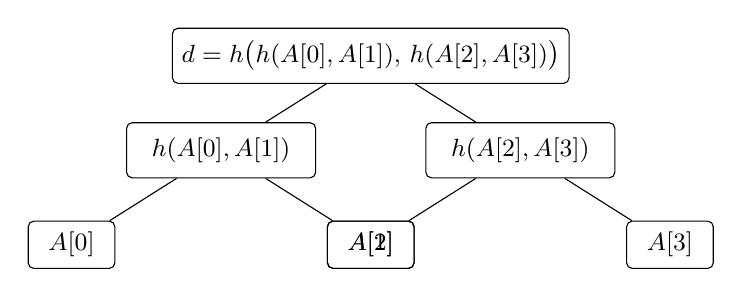
\begin{tikzpicture}[
  level distance=1.2cm,
  sibling distance=38mm,
  every node/.style={font=\small},
  leaf/.style={draw, rounded corners=2pt, minimum width=11mm, minimum height=6mm},
  internal/.style={draw, rounded corners=2pt, align=center, minimum width=24mm, minimum height=7mm}
]
  \node[internal] {$d = h\bigl(h(A[0],A[1]),\,h(A[2],A[3])\bigr)$}
    child {
      node[internal] {$h(A[0],A[1])$}
      child { node[leaf] {$A[0]$} }
      child { node[leaf] {$A[1]$} }
    }
    child {
      node[internal] {$h(A[2],A[3])$}
      child { node[leaf] {$A[2]$} }
      child { node[leaf] {$A[3]$} }
    };
\end{tikzpicture}

\smallskip
\emph{A Merkle tree for a four-element array.  The root is the digest of the
entire array.}
\end{center}

Merkle's original viewpoint was that this turns a fixed-input-length hash
function into a digest for variable-length lists.  In modern applications, the
more important viewpoint is that the root behaves like a short commitment to
the whole array.

\subsection{Authenticated Arrays}

The Merkle-tree construction yields an authenticated array data structure.
The client stores only the root digest, while a storage server holds the full
array and answers read or write queries together with short proofs.

\begin{highlight}[title={Authenticated-Array Interface}]
\[
  \Digest(A) \to d
\]
\[
  \VRead(d, A, i) \to (A[i], \pi_i)
\]
\[
  \VWrite(d, A, i, v') \to (d', A', \pi_i)
\]
\[
  \VerifyAA(d, i, v, \pi) \to \{0,1\}
\]
\end{highlight}

\begin{center}
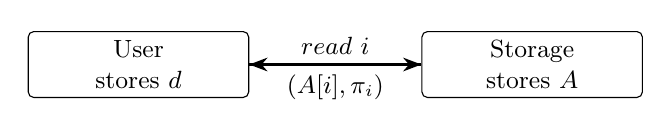
\begin{tikzpicture}[
  every node/.style={font=\small},
  box/.style={draw, rounded corners=2pt, minimum width=28mm, minimum height=8mm, align=center},
  arr/.style={-Stealth, thick}
]
  \node[box] (U) at (0,0) {User\\stores $d$};
  \node[box] (S) at (5.0,0) {Storage\\stores $A$};
  \draw[arr] (U) -- node[above] {$\algo{read}\ i$} (S);
  \draw[arr] (S) -- node[below] {$(A[i],\pi_i)$} (U);
\end{tikzpicture}

\smallskip
\emph{Authenticated-array read query: the verifier stores only the digest and
receives the opened value together with a Merkle proof.}
\end{center}

For a read query, the proof $\pi_i$ is the \emph{co-path} of the queried leaf:
the sibling nodes encountered on the path from the leaf for $A[i]$ to the
root.  Given the claimed value $A[i]$ and these sibling hashes, the verifier
can recompute the root and compare it against the digest $d$ that it stores.

\begin{graybox}[title={Computing a Merkle Read Proof}]
For a query index $i$:
\begin{enumerate}
  \item read the leaf value $A[i]$;
  \item collect the sibling hashes on the root-to-leaf path, i.e. the co-path;
  \item return $(A[i],\pi_i)$, where $\pi_i$ records those sibling hashes in
        the order needed to recompute the root.
\end{enumerate}
\end{graybox}

For a write query, the storage server replaces $A[i]$ with the new value $v'$
and recomputes the hashes on the same root-to-leaf path.  The verifier checks
that the claimed new root $d'$ really is what one obtains by updating the leaf
at position $i$.

\begin{proposition}[Informal soundness of Merkle authentication]
If $h$ is collision-resistant, then the Merkle-tree authenticated-array
construction is sound: an efficient adversary cannot cause the verifier to
accept an incorrect read or write except with negligible probability.
\end{proposition}

\begin{proof}[Proof sketch]
To make the verifier accept a false claim about the contents of the array, the
adversary would have to provide a co-path that recomputes to the correct root
while opening the root to a different leaf value or a different update.  That
forces two distinct inputs to some invocation of $h$ to produce the same
output, yielding a collision in $h$.
\end{proof}

\subsection{Cost of Merkle Authentication}

If the array has $2^k$ cells, then a Merkle proof contains $k$ sibling values,
so the proof length is about $k\ell$ bits.  For example, with $k=64$ and
$\ell=256$,
\[
  k\ell = 64 \cdot 256 = 16384
\]
bits of path data per memory access.

That is far smaller than storing all of memory, but it is not free.  In a
SNARK backend, the path values must still be committed and checked.  The hash
function also matters enormously:
\begin{itemize}
  \item a conventional hash such as SHA-256 can cost on the order of
        $3\times 10^4$ constraints per compression, so a $64$-level path costs
        roughly $1.9$ million constraints;
  \item a SNARK-friendly hash such as Poseidon can be closer to $250$
        constraints per compression, bringing the same path down to roughly
        $1.6\times 10^4$ constraints.
\end{itemize}

Even with a carefully designed hash, long executions can still be dominated by
memory-verification cost.

%-----------------------------------------------------------------------
\section{Proving Memory Accesses with Merkle Trees}
%-----------------------------------------------------------------------

The authenticated-array view embeds directly into the CPU-model transcript.

\paragraph{Initial memory root.}
Assume the initial memory contents are public, for example the all-zero array.
The verifier can compute the initial Merkle root
\[
  d_0 = \Digest_h(A_0)
\]
itself.

\paragraph{Read steps.}
If step $\tau$ reads address $a$ and returns value $v$, then the witness
contains a Merkle opening $\pi_\tau$ for the claim that the current memory root
$d_\tau$ opens at address $a$ to value $v$.  The circuit checks
\[
  \VerifyAA(d_\tau, a, v, \pi_\tau) = 1.
\]
The CPU-step constraints separately check that the opcode semantics use this
same value $v$, e.g. that a load instruction actually places $v$ into the
appropriate register.

\paragraph{Write steps.}
If step $\tau$ writes a new value $v'$ at address $a$, the witness includes the
opening information needed to authenticate the old value and recompute the new
root $d_{\tau+1}$.  The circuit checks that $d_{\tau+1}$ is obtained by
updating leaf $a$ to $v'$ in the tree rooted at $d_\tau$.

Thus each memory access is verified \emph{locally} inside the transcript:
instead of sorting the entire access log, the prover behaves as the storage
server for an authenticated array, and the $\algo{R1CS}$ verifies the resulting
local proof.

\begin{remark}
This method eliminates the global routing-network sort, but it replaces it with
logarithmic-cost cryptographic checks at every memory access.
\end{remark}

%-----------------------------------------------------------------------
\section{Randomized Circuits}
%-----------------------------------------------------------------------

Memory fingerprinting uses a different style of check.  Instead of a purely
deterministic circuit, the verifier provides randomness.

\begin{definition}[Randomized circuit]
A randomized circuit is a circuit
\[
  C(x, w; r)
\]
with public input $x$, witness $w$, and verifier-chosen randomness $r$.  The
soundness guarantee is over the random choice of $r$.
\end{definition}

A randomized circuit is the algebraic analogue of a public-coin
interactive verifier, or equivalently an \algo{MA}-style verifier rather
than an ordinary deterministic NP verifier.

To prove statements about such a circuit in zero knowledge, the prover first
commits to the portion of the witness that does \emph{not} depend on $r$.
After seeing that commitment, the verifier samples $r$ and sends it to the
prover.  The prover then fills in the rest of the witness and proves that
$C(x,w;r)=1$.

\begin{center}
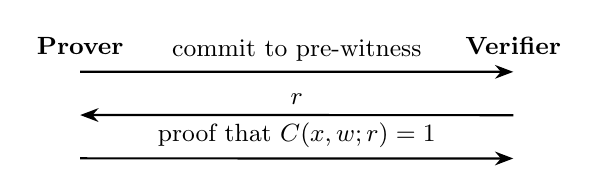
\begin{tikzpicture}[
  node distance=5.5cm,
  every node/.style={font=\small},
  arr/.style={-Stealth, thick}
]
  \node (P) {\textbf{Prover}};
  \node (V) [right of=P] {\textbf{Verifier}};

  \draw[arr] ($(P.south)+(0,-0.1)$) -- node[above] {commit to pre-witness} ($(V.south)+(0,-0.1)$);
  \draw[arr] ($(V.south)+(0,-0.65)$) -- node[above] {$r \getsr \F$} ($(P.south)+(0,-0.65)$);
  \draw[arr] ($(P.south)+(0,-1.2)$) -- node[above] {proof that $C(x,w;r)=1$} ($(V.south)+(0,-1.2)$);
\end{tikzpicture}
\end{center}

If the protocol is public coin, then the extra interaction can itself be
collapsed with Fiat--Shamir by seeding the Fiat--Shamir transcript with the
commitment to the pre-witness.

%-----------------------------------------------------------------------
\section{Memory Fingerprinting}
%-----------------------------------------------------------------------

Memory fingerprinting reduces memory consistency to \emph{multiset equality}.
The randomized-circuit machinery above is the vehicle for proving that equality
efficiently.

\subsection{Reduction to Multiset Equality}

Starting from the execution transcript of $P'$, the memory operations are
transformed as follows.

\begin{enumerate}
  \item Add an initial write to every memory location.
  \item Before every write, insert a dummy read of the same location.
  \item After every read, insert a write-back of the same value to the same
        location.
  \item Whenever a value is written, append the current timestamp to the value.
  \item After the program terminates, add final reads of all memory locations.
  \item If a read returns a timestamp larger than the current timestamp, reject.
\end{enumerate}

The role of the timestamp is to version each memory cell.  If the same address
is written several times, then the corresponding values are no longer confused:
they become distinct versioned values.

The dummy-read and write-back steps put the transcript into a form where
every read and every write can later be matched against a corresponding
versioned memory event.  This yields a reduction to multiset equality.

\begin{remark}
Once memory events are versioned in this way, memory consistency can be
phrased as equality of two multisets of decorated memory accesses rather than
as dynamic consistency of a mutable array.
\end{remark}

%-----------------------------------------------------------------------
\section{Lookup Arguments for Read-Only Memory}
%-----------------------------------------------------------------------

Read-only memory is easier than fully mutable memory.  If the memory table
never changes, then no dynamic write consistency must be maintained, and the
problem is much closer to repeated membership checking in a fixed table.  That
is the natural setting for lookup arguments, which can do better than the fully
dynamic mechanisms above.

The witness in the read-only setting consists of claimed index-value pairs
\[
  (a_1,v_1),\ldots,(a_t,v_t),
\]
and the target statement is that
\[
  T[a_i]=v_i
  \qquad\text{for all } i.
\]
After concatenating or randomly compressing each pair into one field element,
the task becomes repeated membership checking in a public table.

\begin{proposition}[Read-only lookup reduction]
If the memory table $T$ is public and immutable, then read consistency reduces
to proving that each encoded query element belongs to the public table derived
from $T$.
\end{proposition}

\begin{proof}[Proof sketch]
Without writes, there is no versioning issue and no possibility of reading a
stale value from a location that has since changed.  The only remaining claim
is that each reported pair $(a_i,v_i)$ matches the corresponding public table
entry.  After encoding each pair as one field element, this is a table
membership statement.
\end{proof}

This is the setting in which lookup arguments such as \Plookup\ become useful:
the expensive dynamic-memory logic disappears, and the proof system only needs
to certify repeated membership in a fixed public table.

\bigskip
\hrule
\bigskip

\begin{thebibliography}{9}

\bibitem{Merkle87}
  R.~C. Merkle,
  ``A digital signature based on a conventional encryption function,''
  \emph{CRYPTO}, 1987.

\end{thebibliography}

\end{document}
